\subsection{k-d Tree Construction}
\label{sec:kdtree}
% At each step you reason about tradeoffs/alternative design choices and
% justify why you did it in the way you did it (advantages/shortcommings,
% and why your approach is reasonable). Of course mostly related to performance.

% Whenever possible, support your reasoning with (as in point to) experimental
% evaluation results (next).

% - for each have a difficulties / shortcomings section
% - include nice code of each - high level showing the map reduce constructions and such - just pseudocode (simplified version)
%     - it should show the parallel constructs - okay to add sort there from tree construction bc. the text should state that we are using batched mergesort
%     - it's just nice to see the loops and mapping constructions - it doesn't have to be your code, it can be the nice solution before we fixed the tree construct with sort where we split it up etc. 
%         - which will help you, because then you can discuss based on the code like you did in the background. 
%     - it doesn't have to work and it can be incomplete



% of listing \ref{lst:tree} 

	% 3.2 k-d Tree Construction
	% 	"the idea is that we are reducing an irregular problem to a regular problem in terms of parallelism, by means of padding" - such that all parallel operations have the same size such that we can do loop interchange, distribution and so on - to efficiently optimise parallelism. 
	% 	- essential thing: padding technique that allows regular parallelism which is much more efficient since you write the code with regular parallelism and flattening - argue that the proposed solution uses at most 1 more 1 padded element per leaf and the number of points per leaf is typically in the hundreds so it accounts to less than 1% overhead, so its totally feasible, and this overhead allows for a solution that is built on top of regular parallelism - the parallel dimension has the same size over all the elements of the map and so on. 
	% 	 at least one more - it accounts to less than 1% overhead - so it is totally feasible - it allows to build on top of regular parallelism.
	% 	-
	% 	- what is needed to compute so we get a more accurate result: lower bound and upper bound. 
		
	% 	Difficulties: 
	% 		- batch sorting is a detail - shortcomings in compiler - it was not possible to have the sorting inside the map
	% 			- because of some shortcomings in the Futhark compiler, it wasn't able to efficiently exploit the regular parallelism if we put the map on top a mergesort - it didn't manage to interchange and so forth, and the same for radix sort.   
	% 		- not fusing the reduce because then Futhark will fuse them inside. 
	% 			- not fusing the reduces, because if we refused them, then Futhark is not going to also utilise the parallelism inside
		
	% 	- explaining the sorting solution
	% 	- reasoning about choices w.r.t sorting over partition
	% 		- and why are there three inner maps in the for-loop (due to sorting)

% \begin{equation} \label{eq1}
% \begin{split}
% A & = \frac{\pi r^2}{2} \\
%  & = \frac{1}{2} \pi r^2
% \end{split}
% \end{equation}


Listing \ref{lst:tree} represents Futhark-like pseudo-code to demonstrate the overall steps and parallel constructs that are applied in constructing the k-d tree. Note that the structure is not equivalent to the final code, due to some shortcoming of Futhark that are discussed in subsection \ref{sec:treediff}. 
\\[2mm]
% - explain the lower and upper bound inclusion 
% - the structure of the code - what do each stages do and why - reference back to the algorithm from background. 
% Recall the tree construction Algorithm \ref{alg:tree} from section \ref{sec:back}. it uses divide-and-conquer recursion, which is not supported by Futhark since utilises regular parallelism. Thus, the algorithm is rewritten with an outer sequential for-loop, on line 8, and an inner parallel map on lines 14-28. While Algorithm \ref{alg:tree} 
%  that iterates through each level of the tree, starting from the root. 
% The solution that makes up for the divide-and-conquer structure from Algorithm \ref{alg:tree} is that each new level, we compute the current number of nodes per level and number of points per node per level, lines 9-10, such that we can unflatten the arrays containing the reference points and indices to match the number of nodes of the current level, thus being able to map the correct size. 
% Lines 
Recall the tree construction Algorithm \ref{alg:tree} from section \ref{sec:back} using divide-and-conquer recursion, which is not supported by Futhark. The way we account for the divide-and-conquer recursion in Listing \ref{lst:tree}, is by iterating through a sequential loop from level 0 to $h+1$, in line 8, and computing for each level the number of nodes per level and number of points per node per level, lines 9-10, in order to unflatten the arrays containing the reference point data into sections that fit the current number of nodes for each level. This is illustrated in figure \ref{fig:divtree}. Once the reference points are sorted within the bounds of each node, the arrays with reference data will be re-flattened, ready for the next iteration of the for-loop. 

\begin{figure}[H]
\centering
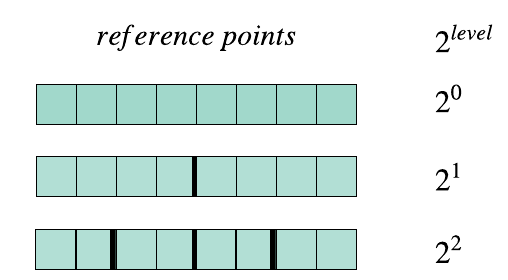
\includegraphics[width=0.4\textwidth]{pics/plot-figs/divtree4.png}
\caption{A demonstration of dividing the reference points at each node level.}
\label{fig:divtree}
\end{figure}

The completed tree will consist of the reorganised array of reference points, the original indices of the reference points and two arrays containing the dimensions with the widest spread and the median values, that together represent the splitting values of each node. In our optimised solution, the tree also consists of two 2D arrays containing the upper and lower bounds for each dimension at each current node. This idea is elaborated further in section \ref{sec:traversal}. 
\\[2mm]
The dimension with the widest spread is computed on lines 16-20, and subsequently, the values in that dimension are sorted, and the reference points and indices are gathered accordingly, on lines 21-24. The median value is picked out on line 25, and both the median and dimension are scattered into the tree arrays containing all medians and dimensions in lines 34-35. Since the upper and lower bounds are computed when finding the dimension with the widest spread, they too are scattered into the tree arrays containing all upper and lower bounds, in lines 36-37. 


\begin{listing}[H]
\begin{minted}{haskell}
entry buildTree [m][d] (points : [m][d]f32) (h: i32) =
    let num_pads =     (...)   -- computing the padding needed
    let padding  = map (...)   -- creating the padding array
    let reference = points ++ padding

    let (ref_idxs, reference, median_vals, median_dims, lower_bounds, upper_bounds) =
    	(...) -- initalising the loop variables
        for level < (h+1) do
            let num_nodes_pr_lvl = 1 << level
            let num_points_pr_node_pr_lvl = m // num_nodes_pr_lvl
            let reference = unflatten num_nodes_pr_lvl num_points_pr_node_pr_lvl reference
            let ref_inds  = unflatten num_nodes_pr_lvl num_points_pr_node_pr_lvl ref_idxs

            let (indices', reference', node_info', lower, upper) = unzip5 <|
                map3 (\i node_arr inds ->
                        let dim_arrs = transpose node_arr   |> intrinsics.opaque
                        let smallest = map o reduce         |> intrinsics.opaque
                        let largest  = map o reduce         -- max numbers for each dim
                        let differences = map         (...) -- computing differences
                        let (dim,_)     = reduce_comm (...) -- dimension w/ widest spread
                        let extract_dim = map         (...) -- extract dimension values
                        let d_sort_idxs = extract_dim |> sort |> map (.0)
                        let indices     = gather d_sort_idxs inds
                        let node_arrp   = gather2D d_sort_idxs node_arr
                        let median      = node_arrp[num_points_per_node_per_lvl // 2, dim]
                        let node_info   = (median, dim)
                        in (indices, node_arrp, node_info, smallest, largest)
                    ) (iota num_nodes_per_lvl) reference ref_inds

            let (medians, dims) = unzip node_info'
            let inds = map (...)   -- computing indices for scatter
            in (flatten ref_idxs', 
                flatten reference', 
                scatter median_vals inds medians,
                scatter median_dims inds dims, 
                scatter2D lower_bounds inds lower,
                scatter2D upper_bounds inds upper)

    in (ref_idxs, reference, median_vals, median_dims, lower_bounds, upper_bounds)
\end{minted}
\caption{Futhark implementation of the tree creation.}
\label{lst:tree}
\end{listing}

% \\[2mm]
% One essential optimisation of the k-d tree construction is the use of padding. Since the datasets might be of sizes that are not dividable with $2^{h+1}$, being the number of leaves, then padding the dataset to match the number of leaves, would allow regular parallelism which is much more efficient, since the parallel dimension will have the same size overall the elements of the map.
One essential optimisation of the k-d tree construction is the use of padding. Since the datasets might be of sizes that are not dividable with the number of leaves, then padding the dataset to match the number of leaves would mean the parallel dimension will have the same size overall the elements of the map, allowing regular parallelism and flattening, which is much more efficient.
\\[2mm]
% Assuming we choose a height that fits that dataset size, such that the number of points per leaf is in the hundreds, it is arguable that the proposed solution uses at most one padded element per leaf,  accounting to less than 1\% overhead. 
Arguably, the proposed solution uses at most one padded element per leaf, accounting to less than 1\% overhead. Assuming that we choose a height that fits that dataset size, such that the number of points per leaf is in the hundreds. 
% It is arguable that the proposed solution uses at most one padded element per leaf, and assuming that we choose a height that fits that dataset size, such that the number of points per leaf is in the hundreds, it accounts to less than 1\% overhead. 
\\[2mm]
The upper bound of the number of pads should not exceed the number of leaves, thus, we want to see how many pads that amount per leaf. 
In Equation \ref{eq:eq1} and \ref{eq:eq2} we denote $n$ to be the total number of reference points, $2^{h+1}$ computes the total number of leaves, where $h$ is the height of the tree excluding the leaves. Thus, $\ceil*{\dfrac{n}{2^{h+1}}}$ denotes the number of points per leaf. In Equation \ref{eq:eq1} we multiply the number of leaves with the number of points per leaf, we get the number of elements that are dividable with the total number of leaves, and by subtracting $n$, we will have the number of pads needed. In Equation \ref{eq:eq2} we divide with the number of leaves on each side, resulting in less than or equal to 1 pad per leaf. 

\begin{align} \label{eq:eq1}
% \textit{number of pads} \leq \textit{number}& \textit{ of leaves} \\[2mm]
\ceil*{\dfrac{n}{2^{h+1}}} \times 2^{h+1} - n   &\leq 2^{h+1} \\[2mm]
\ceil*{\dfrac{n}{2^{h+1}}} - \dfrac{n}{2^{h+1}} &\leq 1 \label{eq:eq2}
\end{align}


\subsubsection{Difficulties and Shortcomings}
\label{sec:treediff}
In the construct above in Listing \ref{lst:tree}, the original solution was to use a merge sort on line 19. However, although it was safe for Futhark to perform a loop distribution and loop interchange between the outer map inside both for loops, it did not realise, in which case the interchange was not performed. Thus, causing poor performance for the tree construction.  The solution was to (1) use batched merge sort, which operates on 2D arrays rather than 1D arrays, (2) distribute the map from line 12, across the body of the map function, such that the sorting is outside the map. 
\\[2mm]
Another shortcoming shows by the use of \texttt{intrinsics.opaque} at lines 14-15 in Listing \ref{lst:tree}, where the purpose is to prevent the Futhark compiler from fusing the two map-reduce compositions on lines 15-16. The reasoning behind this is that both map-reduce compositions call on the same size array, namely m. 
\\[2mm]
Since the Futhark compiler uses moderate flattening, a map-reduce composition will execute in parallel. However, in a map-reduce composition inside a map, as we have in lines 13 and 15-16, the inner map-reduce composition will be sequentialised, and thus resulting in inefficient code. By adding \texttt{intrinsics.opaque} and preventing the fusion, the compiler will create two reduce inside a map, which in return will exploit all parallelism. 


% 272512/256620 = 1,0619281428

% data/brute/10test-k3-d4.in
% [580000][4]f32


% with: 
% dataset data/traverse/13test-k3-d14.in: 97395033.00μs (avg. of 1 runs; RSD: 0.00)
% dataset data/traverse/13test-k5-d14.in: 108650237.00μs (avg. of 1 runs; RSD: 0.00)
% dataset data/brute/2brute2.in:       314551.00μs (avg. of 1 runs; RSD: 0.00)
% dataset data/brute/10test-k3-d4.in:  256620.00μs (avg. of 1 runs; RSD: 0.00)

% without:
% dataset data/traverse/13test-k3-d14.in: 97781445.00μs (avg. of 1 runs; RSD: 0.00)
% dataset data/traverse/13test-k5-d14.in: 108743904.00μs (avg. of 1 runs; RSD: 0.00)
% dataset data/brute/2brute2.in:       319978.00μs (avg. of 1 runs; RSD: 0.00)
% dataset data/brute/10test-k3-d4.in:  272512.00μs (avg. of 1 runs; RSD: 0.00)














% In the construct above in listing \ref{lst:tree}, if we look only at the construct between the \texttt{map3} on line 12 and the merge sort performed on line 19, we would get the following structure.
% if we look only at the construct between the \texttt{map3} on line 12 and the merge sort performed on line 19, we would get the following structure.
% \begin{verbatim}
% 	map 
% 	    for i < d
% 	        for j < i+1
% 	            map f (size n)
% \end{verbatim}

% 	We need to make sure that we are not reversing any of the direction vectors. It cannot start with < (greater than). 

% 	If the outer loop is parallel - then we can interchange always. 

% 	A parallel loop can always be interchanged inside (meaning inwards) - expect in the cases in which the loop index or loop bounds depend on that parallel loop index or on the map. 

% What you would like to do with this code is to interchange the outer map inside both for loops, and then we will have: 
% 	for
% 		for
% 			map
% 				map

% and then we can flatten the two maps and that's done at this point because you have two perfectly nested maps. 


% Fixed by using batched merge sort -> instead of operating on a 1D array we operate on a 2D array, the idea is to distribute the map and you distribute the map across the body of the map function such that you separate the sorting part of it from the rest. 

% So the sorting is outside the original outer map. 

% 	map
% 		map
% 		sort
% 		map

% -> parallel loop distribution and loop interchange. This is what gives you easy flattening for regular cases which is what Futhark s doing. But in this case Futhark is stupid, because it doesn't realise that the inner loop for j ... , since that the bound is i+1 -> it thinks that it cannot interchange the outer map. So it's a Futhark limitation. 


















% \begin{listing}[H]
% \begin{minted}{haskell}
% entry buildTree [m][d] (imB : [m][d]f32) (h: i32) =
%     let num_nodes  = (1 << (h+1)) - 1
%     let num_leaves =  1 << (h+1)
%     let ppl  = (m + num_nodes) / num_leaves  -- ceil(m / (2^(h+1)))
%     let m'   = ppl * num_leaves
%     let num_pads = m' - m
%     let pad = map (\_ -> map (\_ -> f32.inf) (iota d)) (iota num_pads)
%     let imB = imB ++ pad
%     let num_patches_in_leaf = m' // num_leaves
%     let tot_nodes = num_nodes+num_leaves

%     let (ref_idxs, reference, median_vals, median_dims, lower_bounds, upper_bounds) =
%         loop(ref_idxs, reference, median_vals, median_dims, lower_bounds, upper_bounds) =
%           (iota m, points, replicate..., replicate..., replicate..., replicate...)

%         for level < (h+1) do
%             let num_nodes_per_lvl = 1 << level
%             let num_points_per_node_per_lvl = m // num_nodes_per_lvl

%             let (imB_idxs', reference, node_info', lower, upper) = unzip5 <|
%                 map3 (\i node_arr inds ->
%                         let dim_arrs = transpose node_arr   |> intrinsics.opaque
%                         let smallest = map o reduce         |> intrinsics.opaque
%                         let largest  = map o reduce
%                         let differences = map (...) 	-- computing differences
%                         let (dim,_)     = reduce (...)  -- dimension w/ widest spread
%                         let extract_dim = map (...) 	-- extract dimension values
%                         let d_sort_idxs = extract_dim |> sort |> map (.0)
%                         let indices     = gather d_sort_idxs inds
%                         let node_arrp   = gather2D d_sort_idxs node_arr
%                         let median      = node_arrp[num_points_per_node_per_lvl // 2, dim]
%                         let node_info   = (median, dim)
%                         in (indices, node_arrp, node_info, smallest, largest)

%                     ) (iota num_nodes_per_lvl) referencep ref_inds

%             let test = ref_idxs'
%             let (medians, dims) = unzip node_info'

%             let inds = map (...)
%             in (flatten ref_idxs', flatten reference, scatter median_vals inds medians,
%                 scatter median_dims inds dims, scatter2D lower_bounds inds lower,
%                 scatter2D upper_bounds inds upper)

%     in (ref_idxs, reference, median_vals, median_dims, lower_bounds, upper_bounds)
% \end{minted}
% \caption{Futhark implementation of the tree creation.}
% \label{lst:tree}
% \end{listing}

















